\subsection*{Problema 21}
\textbf{Enunciado:} Calcular la integral:
\begin{equation*}
\int \dfrac{2x^2 - 7x - 1}{x^3 + x^2 - x - 1} \, dx
\end{equation*}

\textbf{Solución:} Analizamos el denominador
de la función racional para factorizarlo
por agrupación de términos:
\begin{align*}
x^3 + x^2 - x - 1 &= x^2(x + 1) - (x + 1) \\
&= (x + 1)(x^2 - 1) \\
&= (x + 1)^2(x - 1)
\end{align*}

Planteamos la descomposición en
fracciones parciales con factores
repetidos y lineales:
\begin{align*}
\dfrac{2x^2 - 7x - 1}{(x+1)^2(x-1)} &= 
\dfrac{A}{x+1} + \dfrac{B}{(x+1)^2} \\
&\quad + \dfrac{C}{x-1}
\end{align*}

Multiplicamos toda la ecuación por
el denominador común $(x+1)^2(x-1)$:
\begin{align*}
2x^2 - 7x - 1 &= A(x+1)(x-1) \\
&\quad + B(x-1) + C(x+1)^2
\end{align*}

Evaluamos en valores convenientes de $x$:
\begin{align*}
\text{Si } x = 1 &\implies 2(1)^2 - 7(1) - 1 \\
&= C(1+1)^2 \\
-6 &= 4C \implies C = -\dfrac{3}{2}
\end{align*}

\begin{align*}
\text{Si } x = -1 &\implies 2(-1)^2 - 7(-1) - 1 \\
&= B(-1-1) \\
8 &= -2B \implies B = -4
\end{align*}

Para hallar $A$, evaluamos en $x = 0$
y usamos $B = -4$, $C = -\dfrac{3}{2}$:
\begin{align*}
-1 &= A(1)(-1) + B(-1) + C(1)^2 \\
-1 &= -A - B + C \\
-1 &= -A - (-4) - \dfrac{3}{2} \\
-1 &= -A + 4 - \dfrac{3}{2} \implies A = \dfrac{7}{2}
\end{align*}

Sustituimos los coeficientes $A$, $B$ y $C$
en la integral original:
\begin{align*}
&\int \dfrac{2x^2 - 7x - 1}{x^3 + x^2 - x - 1} \, dx = \\
&\int \left( \dfrac{7/2}{x+1} - \dfrac{4}{(x+1)^2} - \dfrac{3/2}{x-1} \right) dx
\end{align*}

Integramos cada término por separado:
\begin{align*}
&= \dfrac{7}{2} \ln|x+1| + \dfrac{4}{x+1} \\
&\quad - \dfrac{3}{2} \ln|x-1| + C
\end{align*}

Agrupamos los logaritmos utilizando las
propiedades correspondientes:
\begin{align*}
&= \dfrac{7}{2} \ln|x+1| - \dfrac{3}{2} \ln|x-1| \\
&\quad + \dfrac{4}{x+1} + C \\
&= \dfrac{1}{2} \ln\left| \dfrac{(x+1)^7}{(x-1)^3} \right| \\
&\quad + \dfrac{4}{x+1} + C
\end{align*}

\begin{figure}[H]
	\centering
	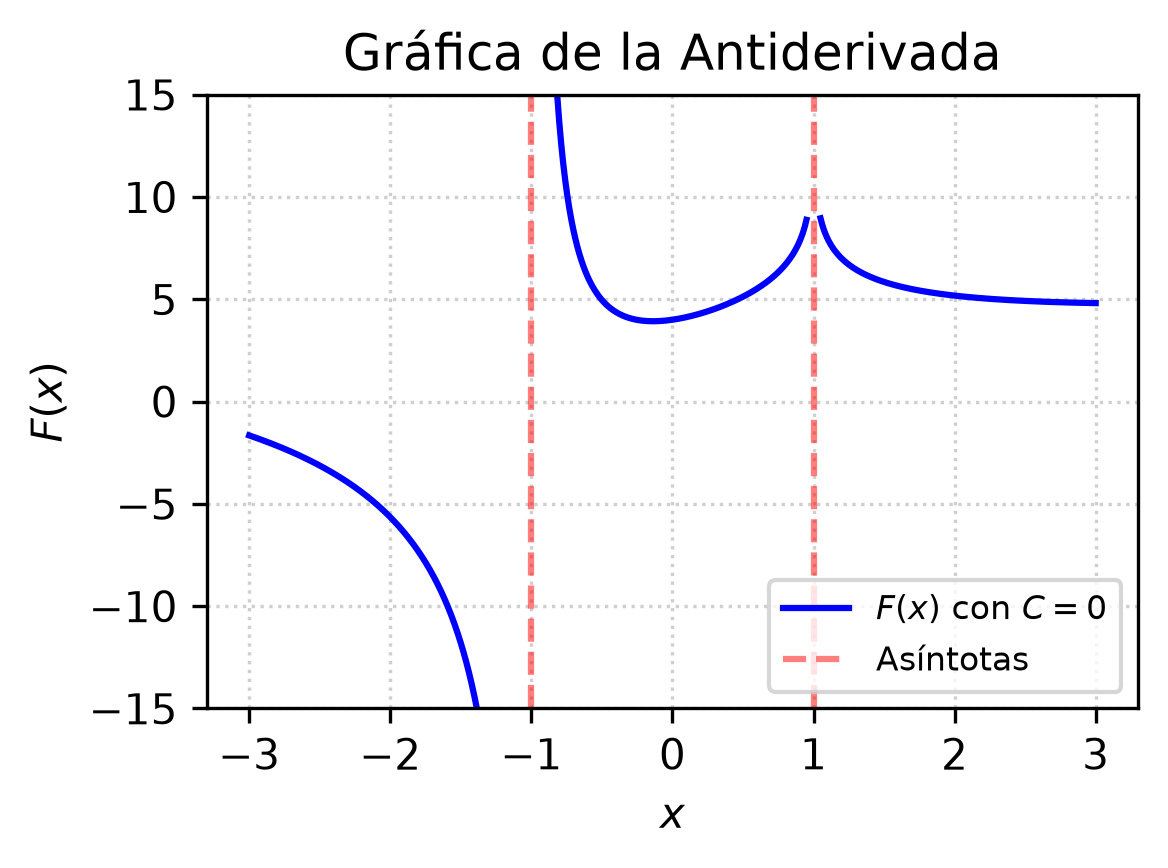
\includegraphics[width=\columnwidth]{semana_03/graficas/SEM03_P21_grafica.png}
	\caption{Representación gráfica de $f(x)$ y su antiderivada $F(x)$ evaluada para la constante de integración $C = 0$ (Problema 21).}
	\label{fig:problema21}
\end{figure}
